% 1_introduction.tex

\cleardoublepage
\chapter{Introduction}


  

  		
  	In recent years, the space sector has seen a significant shift in the paradigm of space launch system design. 
  	The sector has moved towards privatisation, with new and innovative launch systems competing to offer the most cost-efficient and reliable launches. 
  	The sector has also seen a split between those who produce large satellite launchers and those who produce small satellite launchers.
  	For large payload launchers, reusability is a major focus in the design of new launch systems, with the purpose of making a launch system cost efficient over multiple launches\cite{Faa2018}. 
  	For small payload launchers, reusability is more complex than for large launchers, as the additional systems necessary for reusability add a larger fraction of system mass, and require a proportionally larger fuel mass. 
  	Consequently, the focus of small launch system design is currently on producing expendable launch systems as cheaply and efficiently as possible, using state of the art technologies such as 3D printing to expedite the process and minimise cost\cite{Niederstrasser2015}.
  	However, if reusability is able to be successfully integrated into small launch system design, it has the potential to increase the cost efficiency and launch flexibility, potentially opening up the small satellite market significantly. 
  	
  	
  	
  	A potential candidate for integrating reusability into small satellite launch systems is the use of airbreathing engines\cite{Smart2009a,Ketsdever2010}.
Airbreathing engines produce higher specific impulse than rockets, and do not require oxidiser to be carried on-board a launch vehicle\cite{Smart2010}.  	 
  	The higher efficiency and reduced propellant mass of airbreathing vehicles allows the additional mass of the systems necessary for reusability to be mitigated\cite{Curran2003}. An airbreathing vehicle can be designed in a similar fashion to a conventional aircraft, with wings, stabilisers and ailerons\cite{Shaughnessy1990,Preller2017b}. This type of vehicle has a high lift-to-drag ratio, and good manoeuvrability, allowing for a return flight and landing on a conventional landing strip\cite{Preller2017b}, enabling a fast turn-around and cost-efficient re-use. 
  	
  	The primary high-speed airbreathing engines in consideration for launch vehicles are ramjet and scramjet engines, \textcolor{black}{along with rocket-based combined cycle engines that combine multiple engine cycles for operation over a wider range of flight conditions}\cite{HeiserWilliamPratt1994,Kors1988}. These engines offer good efficiency and have operational regimes that allow them to effectively accelerate a launch vehicle over a range of Mach numbers. 
  	Ramjets and scramjets rely on the high speed of the aircraft to compress the flow of air entering the engine before combustion.  Ramjets slow the air to subsonic speeds before combustion and are limited to operation at low Mach numbers, whereas scramjets keep the flow supersonic throughout, and operate within the hypersonic regime, above Mach 5. 
  	These engines have limited operational regimes, and require atmospheric flight in order to intake air as oxidiser. These operational constraints mean that a launch system cannot be solely powered by airbreathing engines. Rocket power is necessary for at least the exoatmospheric portion of the trajectory. As a result, the designs of airbreathing launch systems require rocket stages to reach orbit\cite{Smart2009a}, \textcolor{black}{and if high-speed airbreathing engines are used in the launch system}, rocket power is also desirable for accelerating scramjet accelerator to minimum operational speed, as the alternative is using \textcolor{black}{different types of lower-speed airbreathing engines sequentially}\cite{Smart2009a}, which is weight and cost intensive. 
  	
  	\textcolor{black}{These various propulsion systems may all be integrated into a single-stage-to-orbit spaceplane that is capable of launching, placing payload in orbit, reentering, and returning to a suitable landing site\cite{Argus,Powell1991,Trefny1999,Roche2000,Pescetelli2012,Young2006,Bradford2000,Hyperion}. Single-stage-to-orbit launch vehicles are fully-reusable, and have the potential to be extremely cost-efficient, if they are able to be reused for many missions\cite{Mcclinton2008}. However, their development cost is likely to be very high, and they are generally suited for launching large amounts of payload-to-orbit\cite{Argus,Powell1991,Trefny1999,Roche2000,Pescetelli2012,Young2006,Bradford2000,Hyperion}, a market which is now extremely competitive thanks to the relatively recent advent of large, partially reusable, rocket-based launch systems. Alternatively, the launcher may be separated into multiple stages, similarly to typical, fully rocket-based launch systems\cite{Wilhite1991,Fujikawa2017,Mehta2001,Takahashi1997,Aberleen,Germain2001,Eklund2012,Bradford2002,Kimura1999,Preller2018a}. Multi-stage airbreathing launch systems have the potential to bring cost-efficient reusability to small payload launchers\cite{Preller2017b}, particularly if they are able to stage at high speeds\cite{Mcclinton2008}. Airbreathing systems scale more efficiently than rockets, meaning that the systems needed for reusability in a small launcher do not require the launcher system to be dramatically increased in size, one of the primary limitations on reusability in small rocket-based launch systems. For this reason, partially-reusable two and three-stage airbreathing launch systems are being investigated for small satellite launch\cite{Preller2017b}. To date, studies have been focussed on two-stage launch systems, however, three stage airbreathing launchers have recently been espoused as potentially offering advantages in reusable mass and mass-to-orbit efficiency\cite{Preller2017b}.}
  	
  	\textcolor{black}{There are as of yet no airbreathing launch systems that have progressed past the research and very early design stages\cite{Argus,Powell1991,Trefny1999,Roche2000,Pescetelli2012,Young2006,Bradford2000,Hyperion,Wilhite1991,Fujikawa2017,Mehta2001,Takahashi1997,Aberleen,Germain2001,Eklund2012,Bradford2002,Kimura1999,Preller2018a}. The development and analysis of trajectories is a crucial part of this early design process, and it is a complex task to ensure that an airbreathing launch system is able to survive launch and fly with maximum efficacy.}
  	 A trajectory must be calculated that allows the launch system to achieve its objective of placing the maximum payload into orbit, while recovering any reusable stages and adhering to the operational limitations of the vehicle\cite{Bulirsch1995}.  
  	\textcolor{black}{ In order to maximise the efficiency of the launch system, and thus the payload-to-orbit, there are complex trade-offs in the performance of the launch system that must be taken into account:} the airbreathing engines of a ramjet or scramjet-powered stage require high dynamic pressure to operate effectively, and airbreathing stages are generally designed for high lift-to-drag. Conversely, rocket-powered stages operate more efficiently at higher altitude, and are generally designed for weight and cost efficiency. For airbreathing launch systems, the various \textcolor{black}{distinct operation modes and phases involved} during launch require trade-offs in engine efficiency and thrust generation, stage mass, and vehicle aerodynamics. These factors \textcolor{black}{result in a complex flight path that does not follow simple design rules for optimal efficiency, requiring advanced trajectory studies to ensure that the launch vehicle is operating effectively.}
  	 
  
  	 \textcolor{black}{
  	   For single-stage-to-orbit airbreathing launch systems, trajectories have been developed and studied in detail\cite{Argus,Powell1991,Trefny1999,Roche2000,Pescetelli2012,Young2006,Bradford2000,Hyperion}, in particular due to a multitude of studies in the 1980s and 90s, the most prominent of which was the National Aerospace Plane (NASP), which led, in part, to the Hyper-X program and the X-43 flight experiment\cite{Mcclinton2008}. These studies show complex trade-offs that occur in maximum efficiency airbreathing vehicle trajectories, including trade-offs between the operational efficiencies of the various engine modes. These trajectories often show flight at maximum dynamic pressure or maximum thermal loading, to maximise the efficiency of there airbreathing engines, before a pull-up to orbit, sometimes initially under airbreathing power. These trajectory analyses generally assume that return is possible, due to the high speed and manoeuvrability of the vehicles allowing flexible reentry, and their on-board low-speed engines allowing propulsion and cruise in-atmosphere. 
  	}
  	
  	   \textcolor{black}{
  	  Compared to single-stage airbreathing systems, multi-stage airbreathing launch system trajectories are far more complex, with even more complex trade-offs between the operational modes due to these modes being separated into mechanically distinct stages\cite{Bulirsch1995}.   	  
  	  There is considerable disparity between studies of two-stage-to-orbit airbreathing launch system trajectories, with significant differences in the shape of the airbreathing flight\cite{Wilhite1991,Fujikawa2017,Mehta2001,Takahashi1997,Aberleen,Germain2001,Eklund2012,Bradford2002,Kimura1999,Preller2018a}.
  	  The return trajectories of two-stage-to-orbit launch systems are generally performed under cruise power, utilising turbojet, or sometimes ramjet engines\cite{Wilhite1991,Mehta2001,Eklund2012,Bradford2002}, or alternatively landing at a point downrange\cite{Takahashi1997}.  No studies have attempted a detailed investigation into the trajectory-based performance trade-offs between the stages, and the maximum efficiency trajectories of two-stage airbreathing launch systems are not well understood. 
  	   For three-stage-to-orbit launch systems the launch trajectory is more complex again, due to there being two separation points at which to consider trade-offs, and each stage generally only having a single engine type. 
  	   The presence of a first-second stage separation, high second-third stage separation speeds, lack of low speed engines on the second stage, and small third stage rocket make the calculation of an optimal trajectory shape for a three-stage airbreathing launcher a unique problem, with extremely complex trade-offs. The study of two-stage-to-orbit trajectories is somewhat useful in this regard, however; the disparity between the various studies that have been conducted, and the absence of inquiry into the performance of the launch system stages, means that detailed investigation of the trajectories of multi-stage vehicles is needed. 
  	   Three-stage-to-orbit systems are by far the least studied of the airbreathing launcher configurations, and have to this point only been designed around the flight of prescribed trajectory shapes that constrain the hypersonic airbreathing stages to constant dynamic pressure\cite{Kimura1999,Preller2018a}. It is currently unknown what the optimal trajectory shape for a three-stage launcher is, whether it is possible to return the second stage of a launch system of this type to its initial launch location, and how the design of the launch system may affect the trajectory shape. 
  	}
  	   
  	     	  	\begin{figure}[ht]
  	     	  		\centering
  	     	  		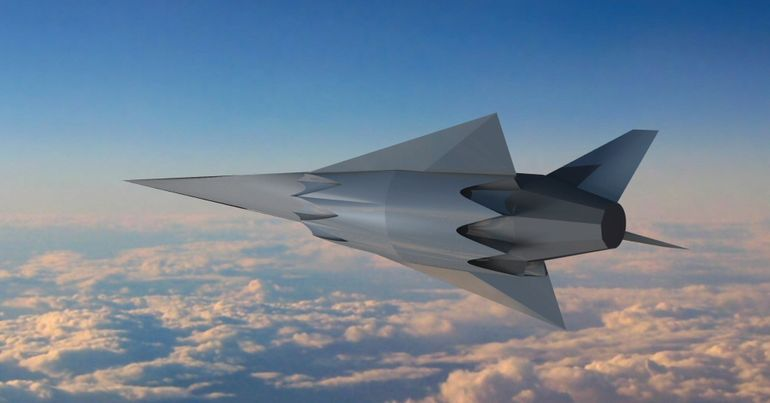
\includegraphics[width=0.6\linewidth]{figures/1_introduction/project-spartan}
  	     	  		\caption{The SPARTAN scramjet-powered accelerator\cite{BBC}.}
  	     	  		\label{fig:project-spartan}
  	     	  	\end{figure}
  	   \textcolor{black}{
  	   This work aims to expand our knowledge on the operation of airbreathing launch systems by developing and analysing optimal trajectories for a partially-reusable rocket-scramjet-rocket small satellite launch system. For this study a launch system design is produced, based on the design of the SPARTAN launch system under development by The University of Queensland and Hypersonix\cite{Preller2017b}.
  	   Optimised trajectories are developed using state-of-the-art optimal control theory techniques that are able to calculate the optimised trajectory profile for a launch vehicle in a robust and computationally efficient manner, allowing a trajectory to be calculated in which the flight path of each individual stage is considered simultaneously to produce a maximum-payload trajectory\cite{Betts1998}. 
  	   Optimal control is able to produce an optimised trajectory that satisfies the specific structural and flight constraints of the vehicle being simulated, allowing the physical limitations of each vehicle  to be imposed\cite{Betts1998}.
  	   This work gives insights into the trade-offs between the rocket and airbreathing stages that are unique to this type of launch system. This manner of optimal trajectory analysis allows for generalities to be made about the nature of the trajectory shape, and for the performance of the launch system to be investigated in order for the understanding of three-stage airbreathing launch systems to be improved.
  	   This trajectory analysis is intended to both aid in the ongoing design process of multi-stage launchers, by characterising the performance needs of a rocket-scramjet-rocket launch system throughout its trajectory, as well as to stand on its own merit by indicating the best possible trajectory shape for this type of launch system. 
  	}
  	   
  	   

  	  	
  	  	\newpage
\textcolor{black}{
  \section{Research Goals}
}
\noindent
    The aim of this work is to expand the knowledge and understanding of airbreathing launch systems and their operation, through the development and analysis of optimised trajectories for a rocket-scramjet-rocket three-stage airbreathing launch system. 
    
\vspace*{10pt}
    \noindent This aim will be achieved by addressing the following research goals:
    \begin{enumerate}
    	 \item \emph{Generate new knowledge in regards to the optimal trajectory shape of a three-stage airbreathing launch system flying to space, through the development of a robust and representative maximum efficiency trajectory.}
    	 
    	 A launch system design will be developed, along with a robust vehicle simulation and trajectory optimisation toolkit. Maximum efficiency trajectories will be produced, and investigated in detail to provide insights into the optimal operation of a three-stage airbreathing launch system.  
    	    \\
\item \emph{Improve the understanding of the viability of reusability in airbreathing launch systems, through an investigation of the impact of airbreathing stage fly-back on the optimised trajectory for a three-stage airbreathing launch system. }

The vehicle simulation and optimisation toolkit will be used to investigate the capability for fly-back in a three-stage airbreathing launch system. Maximum efficiency trajectories will be generated with fly-back included, and these will be compared and contrasted to the trajectories without fly-back. A thermal analysis will be conducted to understand the aerothermal effects of the maximum efficiency trajectory on the launch system. 
 \\
      \item \emph{Improve the understanding of how design affects the performance of airbreathing launch systems, and explore the effects of design variations on the maximum efficiency trajectories of airbreathing launch systems, including stage-stage interactions.}
      
      Key design parameters will be varied, and maximum efficiency trajectories produced for each design variation. The effects of varying these parameters on the optimised trajectory and performance of the launch system will be studied, to give insights into the relative magnitude effects of the key design parameters studied, and analyse the sensitivity of the optimised trajectories and stage-stage interaction phenomena under design variations. 
\\
    \end{enumerate}

  \clearpage
  \section{Thesis Outline and Contributions}

    \textcolor{black}{
    \subsubsection*{Chapter 2 - Background}
}
	Contextual background is presented to frame the objectives of this work. Details are provided on the current state of space launch systems to inform on the current developments in the industry, with a particular focus on small satellite launchers. An overview of scramjet engines is provided to illustrate their potential advantages, followed by an outline of the launch system design process to position this work within the conceptual and preliminary design space.

    \subsubsection*{Chapter 3 - Literature Review}
      A review of literature related to the various aspects of this study is presented. The \textcolor{black}{designs and }trajectories of airbreathing launch systems are presented, comparing various \textcolor{black}{single-stage, two-stage and three-stage} conceptual vehicles. \textcolor{black}{It is shown that the optimal flight path for a multi-stage airbreathing launch system has not been well defined, and that for three-stage vehicles the optimal flight path has not been investigated. The SPARTAN launch vehicle is presented in detail, as the most well defined three-stage airbreathing launch system design. The fly-backs and maximum-range trajectories of multiple hypersonic launch systems and gliders are investigated to determine the feasibility of return and the possible trajectory characteristics.} \textcolor{black}{To facilitate the development of an optimised trajectory, }an overview of optimal control techniques is presented, with particular emphasis on the pseudospectral method of solving optimal control problems, which is employed within this study. Lastly, \textcolor{black}{the available methods of aerodynamic analysis are analysed, and details of Cart3D -the computational fluid dynamics tool that is used for aerodynamic analysis in this study- are presented}.
      

    \subsubsection*{Chapter 4 - Modelling of Launch System Dynamics}

      The design of a three-stage launch system is presented, designated the Representative Launch System, and the aerodynamics and engine models of all three stages are detailed. The scramjet accelerator stage, based on the corresponding stage of the SPARTAN, is presented first, followed by the first and third stages. The design of each stage is shown, along with sizing and mass breakdowns. The propulsion model used for each stage is detailed, along with the modelling and interpolation schemes used. The aerodynamic characteristics and simulation methodology of each stage is presented, and the process for trimming each vehicle is specified. \textcolor{black}{Finally, the modelling simplifications present in the design are discussed.}
      
      
      \subsubsection*{Chapter 5 - Trajectory Modelling and Optimisation}
      
      The method used for the simulation and optimisation of the trajectory is presented, including the details of the trajectory analysis program, LODESTAR, that has been developed for this study. The specifics of the optimal control methodology are presented. The simulation methodology is detailed, along with the construction of the optimal control simulation for the mission used in this study. The specific set-up of the optimal control program is detailed for each trajectory stage, specifying the costs and constraints that drive the optimal control solver. Finally, the methods for analysing and validating the final solutions are specified, including energy and thermal analysis.
      
      \subsubsection*{Chapter 6 - Optimised Ascent Trajectory}
      
Maximum payload-to-orbit optimised trajectories for the Representative Launch System, calculated using LODESTAR, are presented. \textcolor{black}{These trajectories represent the first optimised trajectories that have been developed for a three-stage airbreathing launch system.} A trajectory is designed in which the scramjet accelerator is constrained to flight at a constant dynamic pressure, for comparison to prior work. Next, this constraint is released, a maximum payload-to-orbit trajectory is created, and it is found that an increase in altitude at the stage separation points significantly improves payload-to-orbit.
 This trajectory is compared and contrasted to the constant dynamic pressure trajectory to determine the sources of the performance increase. \textcolor{black}{Crucial performance parameters are analysed, including the energy usage of each stage of the launch system, the first time that a multi-stage airbreathing launch system trajectory has been analysed to this level of detail.} 
 Key vehicle design parameters are varied, and the trends in maximised payload-to-orbit and trajectory shape are analysed to study the relative impact of the design parameters on the performance of the launch system. 
 
 
      
      \subsubsection*{Chapter 7 - Optimised Trajectory Including Fly-Back}
      
      The trajectory of the launch system is optimised for maximum payload-to-orbit, including the fly-back of the scramjet accelerator to its initial launch location. \textcolor{black}{This trajectory represents the first time that the fly-back of a stage under scramjet power has been modelled, and the first time that the optimised trajectories of a three-stage system have included fly-back}. 
      It is found to be necessary to reignite the scramjet engines during the return flight, and the scramjet accelerator is found to bank during acceleration to lessen the fuel consumed during fly-back.
      The trajectories with, and without, fly-back are compared to determine the impact of scramjet accelerator fly-back on the performance of the launch system, along with key performance parameters. 
      In a similar fashion to Chapter 5, the effects of vehicle parameters on the optimised trajectory are studied. The sensitivity of the optimised trajectory and payload-to-orbit are analysed, with emphasis on how the fly-back trajectory is affected by the varied vehicle parameters.
      \textcolor{black}{The thermal effects of the maximum payload-to-orbit trajectory on the launch system are investigated, and the impacts of various TPS design parameters are studied.}
     
      

    \subsubsection*{Conclusions and Recommendations}

      The body of this thesis concludes by summarising the most significant findings from this work. Recommendations for future work are made. 
      
      
      
      \chapter{Background}
      
  Launch system technologies have progressed rapidly over the last 60 years. The materials, propulsion technology, aerodynamics and guidance algorithms have all improved significantly, enabling  rockets to become more efficient, cheaper to produce, and more reliable.          
  As the demand for satellite launches grows, and the cost of development of launchers becomes cheaper, the potential for profiting from space launches increases. 
  \begin{figure}[ht]
  	\centering
  	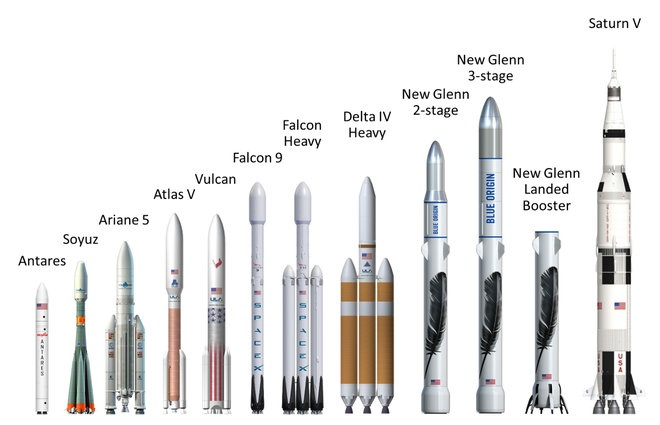
\includegraphics[width=0.9\linewidth]{figures/2_literature-review/LaunchVehicles}
  	\caption{Comparison of Blue Origin and SpaceX partially-reusable launch systems with existing and historic launch systems\cite{BlueOrigin}.}
  	\label{fig:LaunchVehicles}
  \end{figure}
  This has driven a large portion of the space flight industry to move towards privatisation, with a heavy focus on reusable technologies. 
         
    
    Launch vehicles with reusable elements have been in service for many years, in the form of the space shuttle. However, the space shuttle program was hindered by large launch costs and operational complexity, and was not a commercial success\cite{Launius2006}. 
    \begin{figure}[ht]
    	\centering
    	\includegraphics[width=1\linewidth]{"figures/2_literature-review/FalconTrajectory"}
    	\caption{The trajectory of the Falcon Heavy\cite{FalconHeavy}.}
    	\label{fig:FalconTrajectory}
    \end{figure}
    Recently, reusable launchers have become the focus of many of the largest private launch companies, as reusability becomes more achievable due to technological advances\cite{Foust2018,Mosher2018}. The SpaceX Falcon 9 and Falcon Heavy have been demonstrated on multiple occasions, landing booster stages successfully, and re-flying reused boosters multiple times\cite{Foust2018}. In the near future the Blue Origin New Glenn is planned\cite{Foust2018}, with potentially the Airbus Adeline to follow (to be used on the Ariane 6)\cite{Adeline}. The Falcon and New Glenn launchers are large rockets, and are shown in Figure \ref{fig:LaunchVehicles} in a size comparison with other, expendable rocket systems, including the Ariane 5, which is projected to be similarly sized to the Ariane 6. 
     

    
    
    
    
    
    \begin{figure}[ht]
    	\centering
    	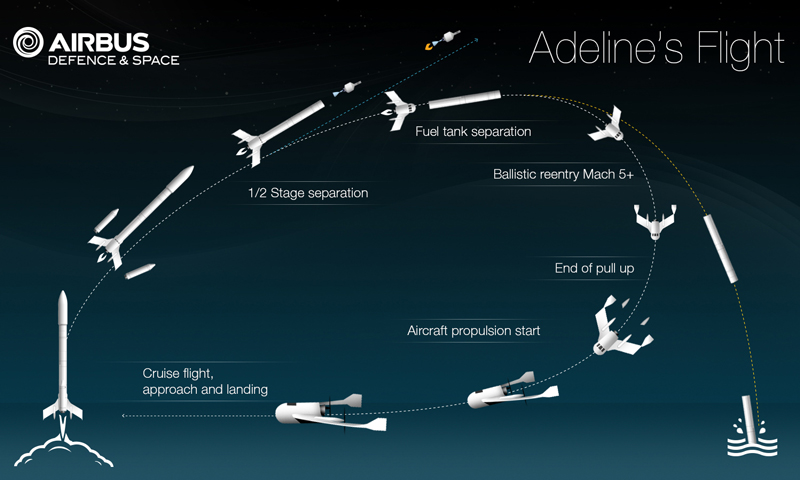
\includegraphics[width=0.7\linewidth]{figures/2_literature-review/visuel_adeline1}
    	\caption{The trajectory of the Ariane featuring Adeline\cite{Adelineb}.}
    	\label{fig:visuel_adeline1}
    \end{figure}
    
    The purpose of reusing launch vehicles is to reduce the cost-over-time of the reused components drastically, which subsequently allows the cost of individual launches to be reduced\cite{RichardWebb2016}. Reducing costs lowers the barrier of entry for space launches, potentially improving the diversity of space-based enterprises. 
    Reusing launch system components also allows faster turnaround times for launches, as refurbishment of stages is much faster than manufacturing stages from scratch. Reduced turnaround times are key for improving mission scheduling, allowing satellites to be launched more rapidly, on a more flexible time frame. 
    For a launch vehicle to be reusable, it must necessarily have the ability to come back to Earth safely, without damage to major system components. In addition, it is preferable for the vehicle to return to its initial launch site, to reduce the cost and time necessary for transport. The trajectories of the Falcon Heavy and Adeline are shown in Figures \ref{fig:FalconTrajectory} and \ref{fig:visuel_adeline1}, \textcolor{black}{ illustrating two radically different approaches to reusability; the exoatmospheric manoeuvre and booster-deceleration of the Falcon; and the in-atmospheric fly-back of the Adeline, which only recovers the engine component of the system. While these reusability approaches use different technologies, they are aiming to achieve the same thing: the recovery of a significant portion of the launch system, with as much of the launch system as possible returned to the initial launch location.} These return flights require the addition of system components, in order to allow the reusable stage to fly to a specified landing point. Control surfaces\cite{Clark2018}, structural components\cite{Sarigul2003}, additional fuel\cite{Sarigul2003}, and in the case of the Adeline, additional engines\cite{Adeline}, must be incorporated within the reusable launch vehicle designs. The weight that these components contribute further increases the fuel and structural mass necessary to initially accelerate the reusable stage. The impact of reusability on the mass and cost of the vehicle is minimised when the speed at the initiation of the return trajectory is decreased. Because of the mass penalties inherent in any reusable stage, most current reusable launch vehicle designs include only reusable first stages, with later stages being expendable. 
    
    
    
    
    \section{Small Satellite Launchers}\label{subsec:smallsats}
    
    
    
    \afterpage{
    	\begin{landscape}% Landscape page
    		\begin{table}
    			
    			\begin{tabularx}{\linewidth}{|X|X|X|X|X|X|X|X|}
    				
    				\hline  \textbf{Launcher} & \textbf{Company} & \textbf{Country} & \textbf{Payload Capacity} & \textbf{Cost/Kg} (USD) & \textbf{Availability }& \textbf{Stages \& Propulsion} & \textbf{Reusability}  \\ 
    				\hline  Electron\cite{Electron} & RocketLab & NZ/USA & 150Kg to SSO & \$32,600 & Available & Rocket-rocket & No  \\ 
    				
    				\hline Bloostar\cite{Bloostar} & Zero2Infinity & Spain & 100kg to SSO & \$40,000 &  - & Balloon-rocket-rocket-rocket & No - Partial Planned\\ 
    				
    				\hline Eris\cite{Gilmour} & Gilmour Space Technologies & Aus& 305kg to LEO  &\$23,000-38,000   & 2022 && No\\ 
    				\hline Intrepid-1\cite{Intrepid} & Rocket Crafters  & USA & 376kg to SSO & \$14400 & Q1 2019 & Rocket-rocket & No \\ 
    				\hline KZ-1A\cite{FT1} & CASIC  &  China & 250kg to SSO  & - & - & Rocket-rocket & No \\ 
    				\hline  Blue Whale \cite{Perigee}& Perigee & Korea & 50kg to LEO & \$4000 & 2021 &  Rocket-Rocket & No\\ 
    				\hline SMILE\cite{Kuhn2017} & NLR &  EU & 50kg & $<$\$50,000 & -  & -& -\\ 
    				\hline 
    				Firefly $\alpha$\cite{firefly}& Firefly Aerospace &  USA & 630kg to SSO & \$9000 & 2020  & Rocket-Rocket& No\\ 
    				\hline 
    				LauncherOne \cite{Virgin} & Virgin Orbit & UK & 200kg to SSO & \$50,000 & 2020 & Aircraft-rocket-rocket & Aircraft\\ 
    				\hline 
    				500R\cite{500R} & Orbital Access  & UK & 500kg to SSO & - & - & Aircraft-Rocket & Fully Reusable \\ 
    				\hline
    			\end{tabularx} 
    			\caption{A selection of the small satellite launchers which are operational or in development.}
    			\label{tab:smallsats}
    		\end{table}
    	\end{landscape}
    }
    
    
    The vast improvements in computational technologies in recent years have allowed satellites to decrease in size and cost to a large degree. These factors have lowered the barrier of entry into small satellite manufacturing significantly, driving a surge in the demand for small satellite launches. Many private and public companies are currently developing small satellite launchers that will allow small satellites to be launched into bespoke orbits on schedules determined by the customer\cite{Faa2018}. The details of a selection of the most promising or innovative of the small satellite launchers currently in active development is shown in Table \ref{tab:smallsats}. Many of these launchers are projected to be available within the next few years, and will offer cost-per-kg comparable to piggybacking on larger launches.
    These small satellite launch systems are mostly expendable, aiming to reduce costs by creating a launch system which is as cost-efficient as possible to produce and launch\cite{Niederstrasser2015}. This often entails making use of conventional, well-tested designs, combined with state of the art manufacturing techniques, such as 3-D printing\cite{Niederstrasser2015,Gilmour}. This method allows for rapid development, although it has an intrinsic cost limit due to the requirement of manufacturing a new launch system for each launch. 
    
    \textcolor{black}{If small satellite launch systems are able to be designed to be reusable, the cost of launch would be able to be brought down further. However, designing a small satellite for reusability is more complex than for a larger rocket system. The systems used to manoeuvre exoatmospherically and decelerate like the Falcon or New Glenn, or fly-back like the Adeline, take up a relatively higher mass margin as the size of the launcher decreases. This in turn increases the mass of the launcher, including the structural mass as well as the fuel and oxidiser mass, relative to other launchers that are targeting the same payload mass range. If a mass and cost efficient design for a reusable small satellite launcher is to be produced, it is likely that a technology must be developed that is specifically geared towards small satellite launch. 
    One of the most promising technologies currently under development that may enable reusable small satellite launch systems is high speed airbreathing engines\cite{Smart2009}, in particular the hypersonic scramjet engine. These engines produce high fuel efficiency and utilise atmospheric oxygen as oxidiser, potentially mitigating the mass inefficiencies caused by the reusability-enabling systems in small launch systems.}
    
 
    
    \section{Scramjets}
    
    A Scramjet, or supersonic combustion ramjet, is an airbreathing engine design that combusts air at supersonic speeds and is capable of high Mach number operation. 
    Across their operating range, scramjets offer much higher specific impulse than rockets, and require significantly less propellant mass\cite{Billig1993,Cook2003}.
    Scramjets were proposed in the 1940's\cite{Curran2001} and found to be capable of positive net thrust in 1993\cite{Paull1993}, but the engines and support systems necessary for commercial applications have yet to be developed. 
    Though scramjets are still in-development, the potential advantages which they offer over rockets for certain applications are driving their development in a number of institutions\cite{Curran2001b}.
    \begin{figure}[ht]
    	\centering
    	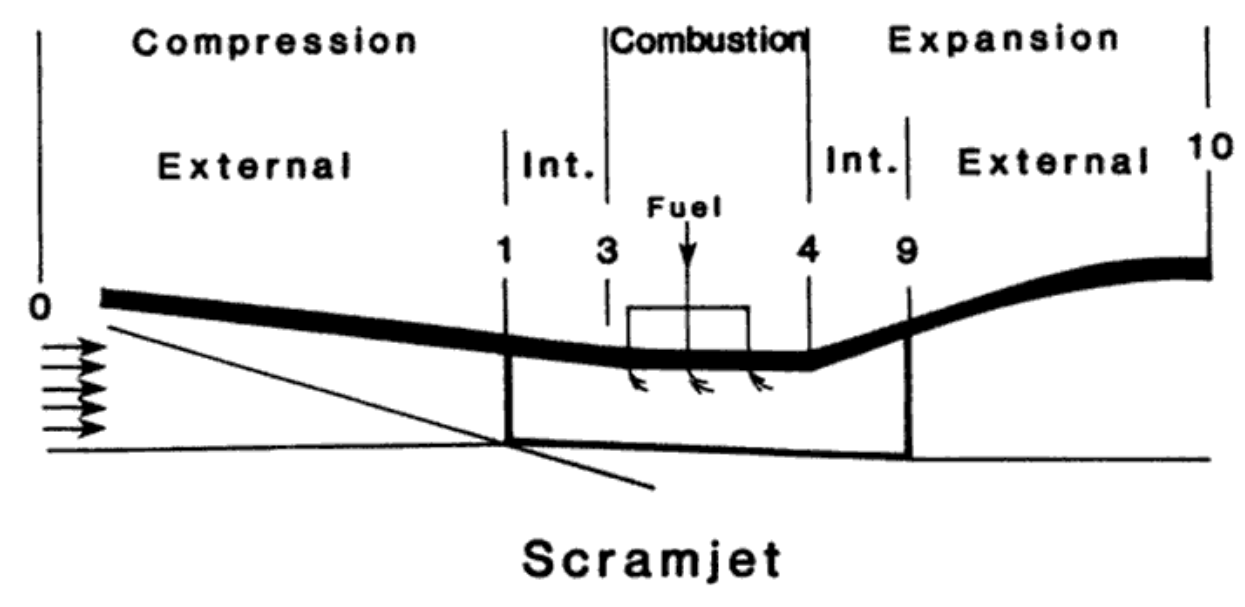
\includegraphics[width=0.7\linewidth]{figures/2_literature-review/scramjet}
    	\caption{A simple schematic of a scramjet engine\cite{Heiser1994}.}
    	\label{fig:scramjet}
    \end{figure}
    
    Scramjets compress air without moving parts, using geometry changes within the engine\cite{Curran2001a}, as well as on the forebody of the vehicle, to create inlet shocks which provide the compression required for combustion\cite{Smart2012}. After combustion, the combustion products are expanded through a thrust nozzle, schematically shown in Figure \ref{fig:scramjet}. This is similar in operation to a ramjet engine, though a scramjet does not generate a normal shock, allowing supersonic air to enter the combustor. Maintaining supersonic speeds throughout the engine allows scramjets to operate with high specific impulse at Mach numbers of 5 and greater. This high specific impulse, along with the usage of atmospheric air as oxidiser, means that a much smaller fraction of a scramjet-powered vehicle consists of propellant mass, when compared to a rocket-powered vehicle\cite{Curran2003}. The smaller fuel mass fraction of a scramjet-powered vehicle mitigates the run-on mass penalties of the vehicle subsystems, allowing features such as wings, control surfaces, landing gear, and passenger transport capabilities to be included in the vehicle design\cite{Curran2003}.  
    
    
    
    
    \begin{figure}[ht]
    	\centering
    	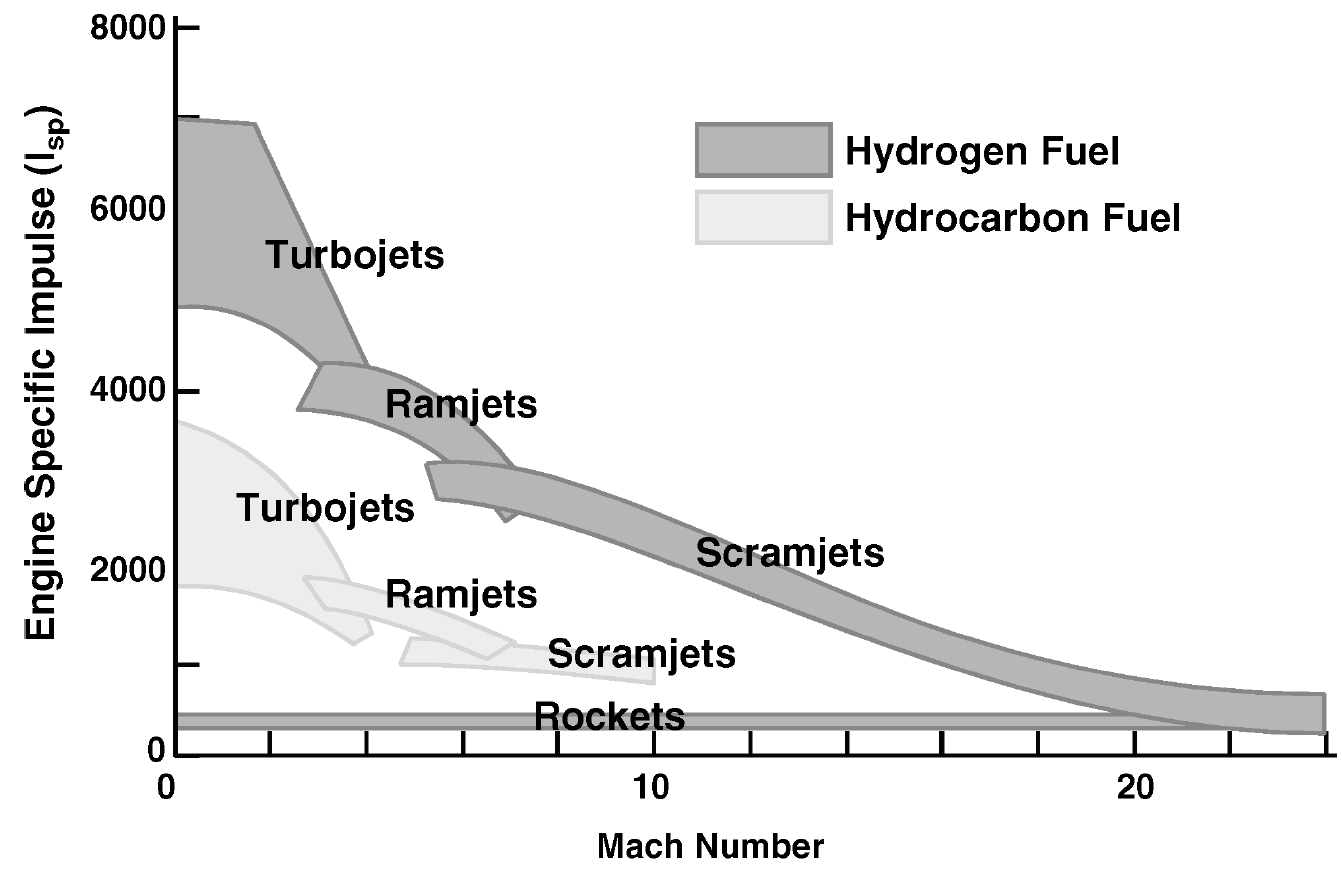
\includegraphics[width=0.7\linewidth]{figures/2_literature-review/Scramjet-Efficiency}
    	\caption{Characteristic performance for airbreathing and rocket engines with Mach number\cite{Fry2004}.}
    	\label{fig:Scramjet-Efficiency}
    \end{figure}
    
    Theoretically, the operable range of scramjets is wide\cite{Smart2007a}. Scramjets are operable at hypersonic speeds around Mach 5, and the specific impulse of a scramjet decreases with speed until it is equal to rockets around Mach 19\cite{Fry2004}, as shown in Figure \ref{fig:Scramjet-Efficiency}. 
    However, in practical designs, the operating range for a scramjet engine is far more limited. 
    For a fixed geometry scramjet, the operable region is constrained by the geometries of the forebody of the vehicle, the inlet, and the combustor of the scramjet engine\cite{Smart2010}.  
    The Mach number range of a scramjet engine varies by design, but Mach number ranges of 5-10\cite{Preller2017b}, 7-11\cite{Dalle2014} and 6-10\cite{Bradford2000} have been suggested as appropriate operable regimes for scramjet-powered launch vehicles.
    The operable range of scramjet engines can be improved with mechanisms to vary the geometry of the inlet during flight\cite{Dalle2011}. However, the systems necessary for variable geometry inlets add weight and complexity to the scramjet engine, and can be detrimental to overall system performance\cite{Smart2010}. 
    
    \textcolor{black}{The inclusion of scramjet engines for high efficiency operation in the hypersonic regime may be considerably advantageous for small satellite launch systems. However, the incorporation of these engines within a launch vehicle requires significant additional design complexity over traditional all-rocket systems, due to their unique operational constraint; the requirement to fly in-atmosphere for long periods, at hypersonic speeds.
    This is a significantly different design philosophy when compared to traditional all-rocket launch systems, which generally want to exit the atmosphere as quickly as possible, and minimise drag losses while doing so. Because of this significant difference in operation, the designs of airbreathing launch vehicles are likely to be radically different from traditional rocket systems. Novel designs must be developed for airbreathing launch systems, that take advantage of the unique advantages offered by airbreathing engines, while overcoming the challenges that they introduce. 
    Currently, the knowledge of how to design launchers incorporating high-speed airbreathing engines is limited, with a particular lack of understanding of the coupling between the design and the associated trajectory to orbit for multi-stage systems. 
    	}
    
    
    
    
    
    \textcolor{black}{
    	\section{The Launch System Design Process}
    }
    %ingo really specfically distinuish airbreatrhing from rocket, ie design is much more complex
    \noindent
    The design of any launch system is a complex, multi-faceted process, that involves many areas of engineering and scientific expertise. Understanding the maximum efficiency trajectory of a launch system and how this interacts with the design is an integral step in the early launch vehicle design. The analysis of a launch system's trajectory enables the designers to understand the performance characteristics and design-trajectory coupling of the launch system, and drives design decisions that are made throughout the development process. 
    
    
     Figure \ref{fig:DesignFlow} illustrates the general design process flow for a launch system as defined by NASA\cite{Blair2001}, in which the design stages involve a repeated iterative process between the overall launch system design and compartmentalised design tasks. This compartmentalisation takes place firstly by separating the
    launch system into its hardware and software subsystems, and then into general areas that define the specifications of the subsystem design (design functions). These areas include;
    \begin{itemize}
    	\setlength\itemsep{.2em}
    	\item aerodynamics;
    	\item trajectory, guidance and navigation;
    	\item control;
    	\item structures;
    	\item thermal;
    	\item propulsion;
    	\item avionics;
    	\item materials;
    	\item and manufacturing,
    \end{itemize}
    among others\cite{Blair2001}. The design is then further compartmentalised into pertinent areas of specific speciality and expertise (discipline functions) that define the problems that must be solved, and skills that are necessary for low level design
    

    The design of a traditional all-rocket launch system may be compartmentalised relatively easily, and the general shape of rocket launch system trajectories are well-known and relatively easily understood.  The primary trajectory goals of a rocket-powered launch system are to minimise drag while not exceeding structural and thermal limits, and in general this results in a vertically-launched pitching trajectory, that exits the atmosphere as rapidly as possible while managing its speed at points of maximum structural and thermal stress. The design and design-trajectory coupling of an all-rocket launch system is relatively well understood, and thus the design process for a rocket-powered launch system is able to be separated into independent stages or subsystems relatively easily, with clear design goals. 
    
   
    
    For an airbreathing launch system, this compartmentalisation is much more difficult, because the design of an airbreathing launch system is much more complex, with significant inter-stage design coupling, and heavy dependencies and trade-offs between the way in which an airbeathing launch system is flown, and its optimal design and performance characteristics. Atmospheric flight of airbreathing stages requires aircraft-style designs for control and stability, and results in complex trade-offs between the performance of the airbreathing engines, and the structural and thermal limitations of each stage. In addition, there is trade-offs between the performance of the various engines that are utilised by airbreathing launch systems, which generally mix airbreathing and rocket engines that have significantly different performance regimes.
    These trade-offs are specific to the types of engines and number of stages being employed by the launch system, and are closely coupled to the trajectory being flown. The investigation of the ideal launch trajectory of an airbreathing launch system, utilising subsystem models of appropriate fidelities, is an integral step in the early design process. Early trajectory analysis is important for the design of the launcher and its subsystems to be investigated, and for significant performance drivers to be identified early on. 
    \begin{figure}[ht]
    	\centering
    	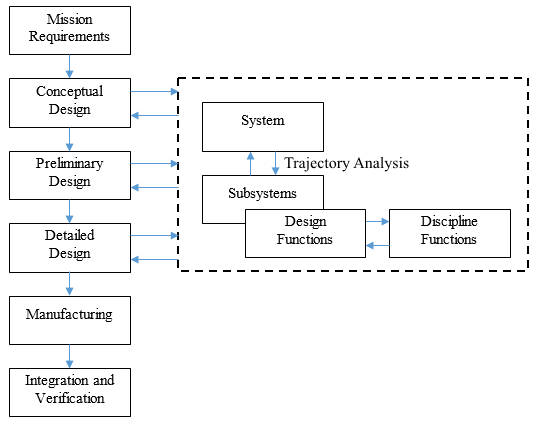
\includegraphics[width=0.6\linewidth]{figures/2_literature-review/DesignFlow}
    	\caption{The general design process flow for a launch vehicle, adapted from Blair et al\cite{Blair2001}}.
    	\label{fig:DesignFlow}
    \end{figure}
  This is particularly true because many of the subsystems and technologies necessary to achieve airbreathing space access are in development at an academic level, and advances are necessary in multiple fields before the flight of an airbreathing launch vehicle becomes a reality. The investigation of the trajectory of an airbreathing launch system gives key insights into the design requirements of the launcher and it subsystems, and can drive academic study on the subsystems of airbreathing launchers, such as their propulsion, control, and thermal protection systems, as well as their overall designs. This can be used by designers to inform early designs, and to reduce the number of iterative cycles required during the design process. 
    
  